% !TEX root = ../intro-stellar-physics.tex

\newcommand*{\bra}[1]{\ensuremath{\left\langle#1\right|}}
\newcommand*{\ket}[1]{\ensuremath{\left|#1\right\rangle}}
\newcommand*{\braket}[2]{\ensuremath{\left\langle#1\right|\left.#2\right\rangle}}

\section{Identical Particles}
\label{s.identical-particles}

As a star contracts, the particles within it are packed ever closer together.  As we saw from our discussion of ionization, the behavior of particles must change when the separation between particles is of the order of the uncertainty in their positions.  Equivalently, our classical description breaks down when the density exceeds roughly
\begin{equation}
    \frac{1\;\textrm{particle}}{(\Delta x)^3} 
    = \left(\frac{\Delta p}{h}\right)^3 
    \sim \left(\frac{m\kB T}{h^2}\right)^{3/2}.
\end{equation}
To investigate this in more detail, let's start by recalling some features of quantum mechanics. We denote a state as $\ket{a}$, where $a$ is just a label.  For example, $a$ could be "electron with such-and-such momentum".  The probability of finding the electron in some other state $\phi$ is given by $|\braket{\phi}{a}|^2$, where $\braket{\phi}{a}$ is a complex number known as the probability amplitude.

Now suppose we have two particles, a and b, and we scatter them so that one particle ends up in detector 1 and the other ends up in detector 2, as shown in Fig.~\ref{f.scattering-classical}. Classically, we would argue that the probability of getting either particle in detector 1 is just
\begin{equation}
    \mathcal{P}(\textrm{a or b in 1}) = \mathcal{P}(\textrm{a in 1}) + \mathcal{P}(\textrm{b in 1}).
\end{equation}
If particles a and b are different---e.g., one is a \carbon\ nucleus and the other is an \oxygen\ nucleus---then this holds in quantum mechanics as well. Quantum mechanically, we would write
\begin{equation}
    \mathcal{P}(\textrm{a or b in 1}) = |\braket{1}{a}\braket{2}{b}|^2 + |\braket{2}{a}\braket{1}{b}|^2.
\end{equation}

\begin{figure}
    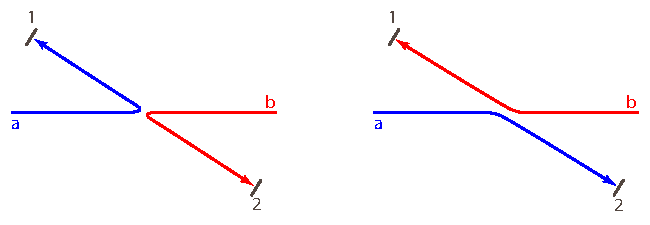
\includegraphics[width=\linewidth]{scattering-classical}
    \caption[Scattering of two identical classical particles]{\label{f.scattering-classical} Scattering of two classical particles, a and b, into detectors 1 and 2.}
\end{figure}

If the particles are identical, however---for example, if a and b are two electrons with identical spin---then the picture in Fig.~\ref{f.scattering-classical} is wrong.  Because of the uncertainty principle, we cannot follow the trajectories of a and b with infinite precision to see which is which; instead, the situation is more like that in Fig.~\ref{f.scattering-quantum}.

\begin{figure}
    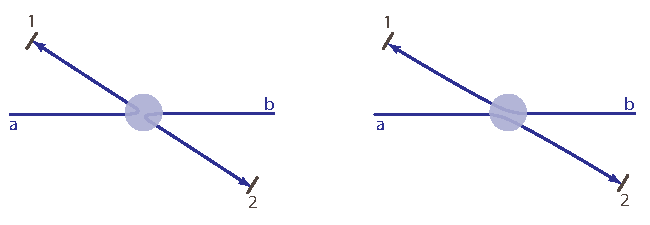
\includegraphics[width=\linewidth]{scattering-quantum}
    \caption[Scattering of two identical quantum particles]{\label{f.scattering-quantum} Scattering of two identical quantum particles.}
\end{figure}

Now, in quantum mechnics if there is more than one, indistinguishable, way of arriving at the final state---in this case, an electron in detector 1 and an electron in detector 2---then we must sum all the amplitudes for getting to the final state, before taking the square. That is, the probabity for this scenario is
\begin{fullwidth}
\begin{eqnarray}
    \mathcal{P}(\textrm{a or b in 1}) &=& |\braket{1}{a}\braket{2}{b} + \braket{2}{a}\braket{1}{b}|^2\nonumber\\
    &=& |\braket{1}{a}\braket{2}{b}|^2 + |\braket{2}{a}\braket{1}{b}|^2 
    + \left[ \braket{1}{a}^*\braket{2}{b}^*\braket{2}{a}\braket{1}{b} + \braket{2}{a}^*\braket{1}{b}^*\braket{1}{a}\braket{2}{b}\right] \nonumber\\
    &=& \mathcal{P}(\textrm{a in 1}) + \mathcal{P}(\textrm{b in 1})
    + \left[ \braket{1}{a}^*\braket{2}{b}^*\braket{2}{a}\braket{1}{b} + \braket{2}{a}^*\braket{1}{b}^*\braket{1}{a}\braket{2}{b}\right].
    \label{e.scattering-quantum}
\end{eqnarray}
\end{fullwidth}
The probability of scattering an electron into detector 1 is the classical value plus the \emph{additional} interference term in $[\cdot]$.

\newthought{To see the effect on the themal properties,} let's imagine putting two particles into the same small volume.  To do this, we imagine the detectors 1 and 2 sliding together until they overlap, as shown in Fig.~\ref{f.fermions}.  Since 1 and 2 are approaching one another, we must have that
\begin{equation}
    |\braket{1}{a}\braket{2}{b}|^2 = |\braket{2}{a}\braket{1}{b}|^2.
\end{equation}
This does not imply, however, that $\braket{1}{a}\braket{2}{b} = \braket{2}{a}\braket{1}{b}$: the amplitudes could differ by a phase factor, so that interchanging the particles would yield
\[
    \braket{2}{a}\braket{1}{b} = e^{i\delta}\braket{1}{a}\braket{2}{b}.
\]
If we interchange the particles, and then interchange them again, we get
\[
    \braket{1}{a}\braket{2}{b} = e^{2i\delta}\braket{1}{a}\braket{2}{b};
\]
since swapping the particles twice just gets up back to the original situation, we must have that $e^{i\delta} = \pm 1$.

\begin{marginfigure}[-8\baselineskip]
    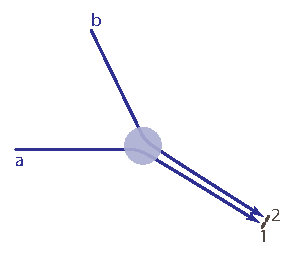
\includegraphics[width=\linewidth]{fermions}
    \caption[Scattering of fermions]{\label{f.fermions}Scattering of two particles into the same position and momentum state.}
\end{marginfigure}

\begin{quote}\itshape
    There are two types of particles: those that change sign under exchage; and those that don't.
\end{quote}

If there is no change of sign, i.e., $\braket{2}{a}\braket{1}{b} = \braket{1}{a}\braket{2}{b}$, then from equation~(\ref{e.scattering-quantum}) we have
\begin{equation}\label{e.boson}
    \mathcal{P}(\textrm{a or b in 1}) = 2|\braket{1}{a}\braket{2}{b}|^2 + 2|\braket{2}{a}\braket{1}{b}|^2.
\end{equation}
This is \emph{twice} the classical value: the probability of the particles entering the same state is enhanced.

In contrast, if $\braket{2}{a}\braket{1}{b} = -\braket{1}{a}\braket{2}{b}$, then equation~(\ref{e.scattering-quantum}) implies that
\begin{eqnarray}
\mathcal{P}(\textrm{a or b in 1}) &=& |\braket{1}{a}\braket{2}{b}| + |\braket{2}{a}\braket{1}{b}| \nonumber\\ 
    && - |\braket{1}{a}\braket{2}{b}| - |\braket{2}{a}\braket{1}{b}| \nonumber\\ 
    &=& 0.\label{e.fermion}
\end{eqnarray}
We cannot have 2 identical particles with the same momentum, position, and spin. 

Particles with integer spin (i.e., their angular momentum is an integer multiple of $\hbar$) have wavefunctions that do not change sign under exchange; these particles are said to obey \emph{Bose-Einstein statistics} (eq.~[\ref{e.boson}]) and are called \emph{bosons}.  Particles with half-integer spin have wavefunctions that do change sign under exchange; these particles are said to obey \emph{Fermi-Dirac statistics} (eq.~[\ref{e.fermion}]) and are called \emph{fermions}.  Photons are bosons; electrons, protons, and neutrons are fermions.

\newthought{To connect with the equation of state,} we begin by imagining a small volume containing $N$ electrons. We divide the phase space into cells,
\[
	\frac{\dif^{3}x\,\dif^{3}p}{h^{3}},
\]
and into each cell we place 2 electrons with opposing spins. We always add the electrons to the lowest open energy level, and repeat the process until we have added all $N$ electrons. This procedure is represented by the equation
\begin{equation}
	N = \frac{2}{h^{3}}\int_{V}\dif^{3}x\int_{0}^{\EF}\dif^{3}p
\end{equation}
In this equation $\EF$, the \emph{Fermi energy}, is the energy of the last electrons added and is the largest filled energy level.

If our volume is isotropic, then we can change variables: first, to spherical momentum coordinates, $\dif^{3}p = 4\pi p^{2}\,\dif p$; second, from $\dif p$ to $\dif\varepsilon$.  Since $p = \sqrt{2m\varepsilon}$, where $\varepsilon$ is the energy of a single electron,
\[
	\dif p = \sqrt{\frac{m}{2\varepsilon}}\,\dif \varepsilon;
\]
we can therefore change variables and integrate over $\varepsilon$ from $0$ to $\EF$ to obtain
\[
	N = \frac{8\pi}{h^{3}}V \int_{0}^{\EF} \sqrt{2}m^{3/2}\varepsilon^{1/2}\,\dif \varepsilon
	= \frac{8\pi}{3h^{3}} V (2m)^{3/2} \EF^{3/2}.
\]
Solving for the Fermi energy gives
\begin{equation}\label{e.fermi-energy}
	\EF = \frac{h^{2}}{2m}\left(\frac{3}{8\pi}\frac{N}{V}\right)^{2/3}.
\end{equation}
What is the total energy of our system? We again integrate over phase space, with each electron multiplied by its energy $\varepsilon$:
\begin{equation}\label{e.total-energy}
	E = \frac{8\pi}{h^{3}}V\int_{0}^{\EF}\sqrt{2}m^{3/2}\varepsilon^{3/2}\,\dif\varepsilon = \frac{8\pi}{5h^{3}}V(2m)^{3/2} \EF^{5/2}.
\end{equation}
Using eq.~(\ref{e.fermi-energy}) to substitute for $\EF$ in eq.~(\ref{e.total-energy}), we can find the energy per unit volume,
\[
	\frac{E}{V} = \frac{3}{5}\left(\frac{3}{8\pi}\right)^{2/3}\frac{h^{2}}{2m}n^{5/3} = \frac{3}{5} n \EF,
\]
where $n=N/V$ is the density of electrons.

Recall that for a non-relativistic gas the pressure is $P = (2/3)(E/V)$.  Hence the pressure of our electron gas is
\begin{equation}\label{e.pressure-electrons}
	P = \frac{2}{3}\frac{E}{V} = \frac{2}{5} n\EF
		= \frac{2}{5}\left(\frac{3}{8\pi}\right)^{2/3}\frac{h^{2}}{2m}n^{5/3}.
\end{equation}
Notice that the pressure is independent of the temperature.

\nocite{Feynman1989The-Feynman-Lec}
